\section{External Interface Requirements}
\label{sec:external_interface_requirements}%

\subsection{User Interfaces}
\label{subsec:user_interfaces}%

\subsection{Hardware Interfaces}
\label{subsec:hardware_interfaces}%
The platform is a web app; this means that it does not require any specific hardware interface except for a computer or any other device with web browser.  
\subsection{Software Interfaces}
\label{subsec:software_interfaces}%
In order to work correctly, the system will need to integrate with a few software components; here they are listed in detail:
\begin{itemize}
    \item \textbf{Database Systems:} To store user profiles, internship details, application records, and feedback securely.
    \item \textbf{Email and Notification APIs:} To send updates and reminders to users about critical events such as deadlines or feedback.
    \item \textbf{Video Conferencing Tools:} For virtual interviews between students and companies.
    \item \textbf{Statistical Analysis Tools:} To extract meaningful data from user interactions and feedback.
\end{itemize}
 
\subsection{Communication Interfaces}
\label{subsec:communication_interfaces}%

\section{Functional Requirements}
\label{sec:functional_requirements}%

\subsection{Requirements}
\label{subsec: requirements}%
\newcounter{h}
\setcounter{h}{0}
\newcommand{\ch}{\stepcounter{h}R\theh}

\begin{center}
    \renewcommand{\arraystretch}{2}
    \begin{longtable}{ l p{0.8\linewidth} } 
        \hline

        \textbf{ID} & \textbf{Description}                                                \\
        \hline
        \ch      & S\&C system allows unregistered users to sign-up.\\
        \hline
        \ch      & S\&C system allows registered users to verify their email address.\\
        \hline
        \ch      & S\&C system allows registered users to login.   \\
        \hline
        \ch      & S\&C system allows registered users to edit their account details.   \\
        \hline
        \ch      & S\&C system allows registered users to delete their account.   \\
        \hline
        \ch      & S\&C system allows registered users to view posted internships on the platform.   \\
        \hline
        \ch      & S\&C system allows registered users to upgrade to a Student account or a Company account. \\                     
        \hline
        \ch      & S\&C system allows registered users to verify their current academic status by validating their institutional email address.\\                     
        \hline
        \ch      & S\&C system allows Students to view available internships. \\  
        \hline
        \ch      & S\&C system allows Students to view available internships ordered by the best matching. \\
        \hline
        \ch      & S\&C system allows Students to receive notification when a new internship matching their profile is posted.\\  
        \hline
        \ch      & S\&C system allows Students to view the details of a specific internship page. \\ 
        \hline
        \ch      & S\&C system allows Students to apply for an internship.\\ 
        \hline
        \ch      & S\&C system allows Students to monitor the status of an application.\\ 
        \hline
        \ch      & S\&C system allows Students to confirm their participation of a scheduled interview.\\
        \hline
        \ch      & S\&C system allows Students to review the agreements of an internship before accepting.\\ 
        \hline
        \ch      & S\&C system allows Students to file a complaint. \\ 
        \hline
        \ch      & S\&C system allows Students to submit feedback after completing an internship.\\ 
        \hline
        \ch      & S\&C system allows Companies to post internship offers by providing detailed information\\ 
        \hline
        \ch      & S\&C system allows Companies to edit an internship's post. \\  
        \hline
        \ch      & S\&C system allows Companies to delete an internship's post. \\  
        \hline
        \ch      & S\&C system allows Companies to review the applications for an internship. \\
        \hline
        \ch      & S\&C system allows Companies to view internship's candidates ordered by the best match. \\
        \hline
        \ch      & S\&C system allows Companies to propose a date to a student to schedule an interview. \\  
        \hline
        \ch      & S\&C system allows Companies to reject a candidate after the interview. \\  
        \hline
        \ch      & S\&C system allows Companies to start an internship. \\  
        \hline
        \ch      & S\&C system allows Companies to view active internships. \\
        \hline
        \ch      & S\&C system allows Companies to file a complaint. \\ 
        \hline
        \ch      & S\&C system allows Companies to submit feedback after completing an internship.\\ 
        \hline
        \ch      & S\&C system allows universities to collect complaints raised by Students.\\ 
        \hline
        \ch      & S\&C system allows universities to collect complaints raised by Companies.\\ 
        \hline
        \ch      & S\&C system allows universities to mediate between Student and Company after a complaint.\\ 
        \hline
        \caption{Requirements}
        \label{tab:worldph_tab}%
    \end{longtable}
\end{center}

\subsection{Use case diagrams}
\label{subsec: use_case_diag}%

\begin{figure}[H]
    \centering
    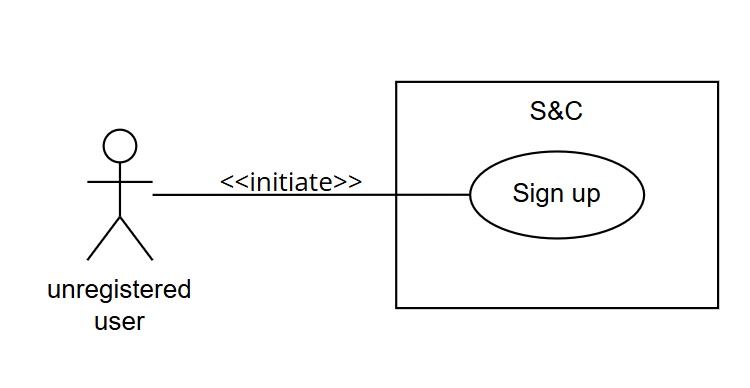
\includegraphics[width=1\linewidth]{Images/use case diagrams/UNREGISTERED_USER.png}
    \caption{Unregistered user}
    \label{fig:enter-label}
\end{figure}

\begin{figure}[H]
    \centering
    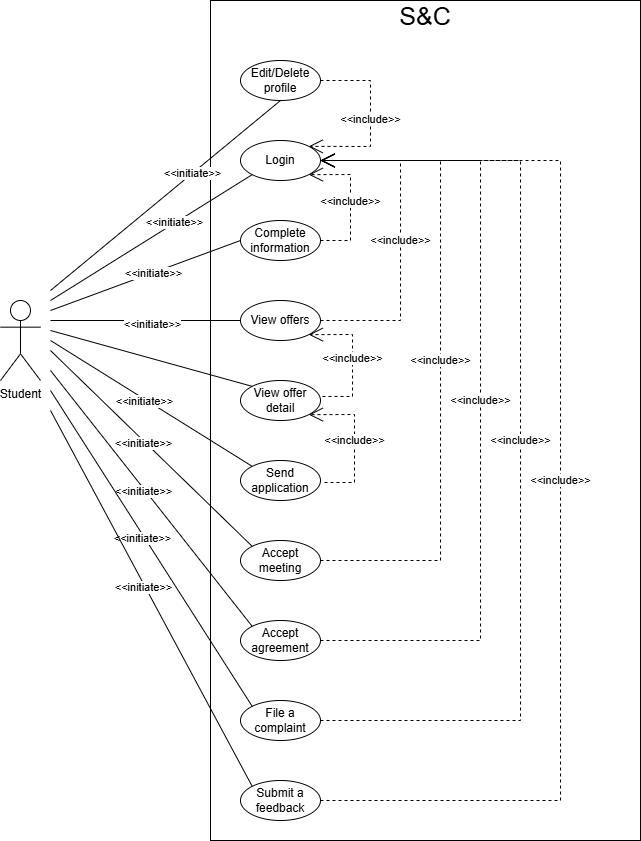
\includegraphics[width=1\linewidth]{Images/use case diagrams/STUDENT.png}
    \caption{Student}
    \label{fig:enter-label}
\end{figure}

\begin{figure}[H]
    \centering
    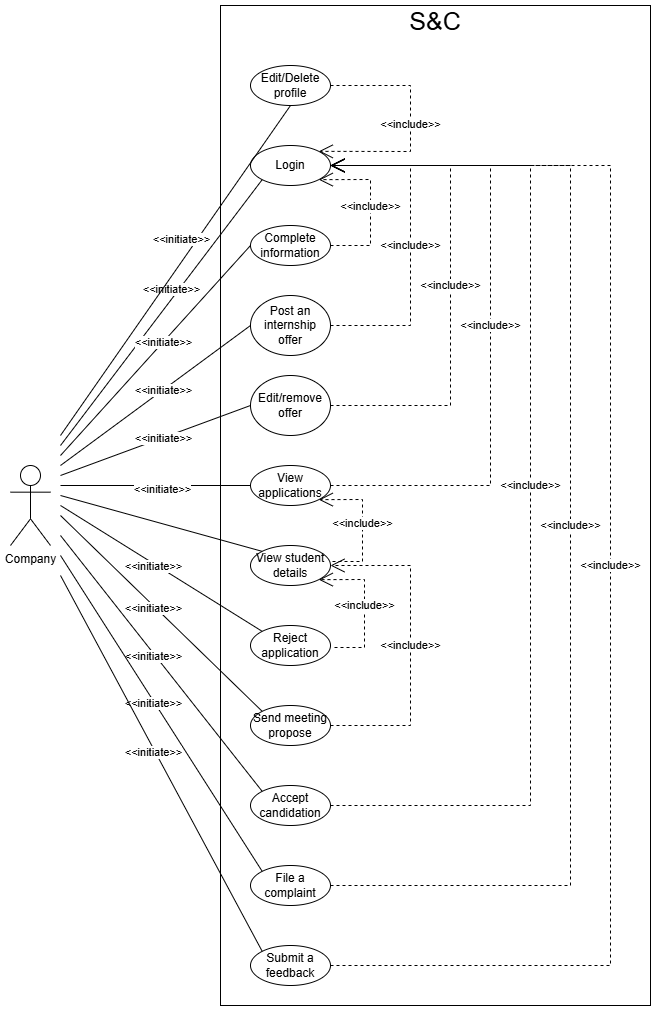
\includegraphics[width=0.9\linewidth]{Images/use case diagrams/COMPANY.png}
    \caption{Company}
    \label{fig:enter-label}
\end{figure}

\begin{figure}[H]
    \centering
    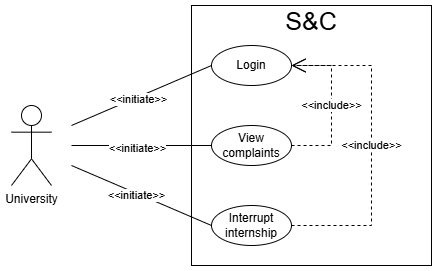
\includegraphics[width=1\linewidth]{Images/use case diagrams/UNIVERSITY.png}
    \caption{University}
    \label{fig:enter-label}
\end{figure}

\subsection{Use cases}
\label{subsec: use_cases}%

\subsection{Mapping on goals}
\label{subsec: map_on_g}%

\section{Performance Requirements}
\label{sec:performance_requirements}%

\section{Design Constraints}
\label{sec:performance_requirements}%

\subsection{Standard compliance}
\label{subsec: standard_compliance}%

\subsection{Hardware limitations}
\label{subsec: hardware_limitations}%

\section{Software system attributes}
\label{sec:performance_requirements}%

\subsection{Reliability}
\label{subsec: reliability}%

\subsection{Availability}
\label{subsec: availability}%

\subsection{Security}
\label{subsec: security }%

\subsection{Maintainability}
\label{subsec: maintainability}%

\subsection{Portability}
\label{subsec: portability}%
